% !TEX root = main.tex

\section{索引与散列} % Chap 11
\subsection{基本概念}
通常索引文件包含记录/索引项,要比原文件小很多
\begin{center}
\begin{tabular}{|c|c|}\hline
search-key & pointer\\\hline
\end{tabular}
\end{center}

两种基本的索引类型:顺序(ordered)索引、散列(hash)索引

\subsection{顺序索引}
\begin{definition}[聚集索引]
在顺序索引中,包含记录的文件按照某个\textbf{搜索码}指定顺序排序,则该搜索码对应的索引称为聚集索引(clustering index),也被称为主索引(primary)。
但注意并\textbf{不是建立在主码上的索引}。
若搜索码指定的顺序与文件中记录的物理顺序不同,则称为非聚集索引(secondary)。
\end{definition}
\begin{definition}[稠密/稀疏索引]
对于每个搜索码都出现索引记录的称为稠密索引,只包含特定搜索码值的称为稀疏索引。
非聚集索引一定是稠密的。
\end{definition}

稀疏索引查找方法即找到最大搜索码键值小于$K$的,然后继续往下搜索。
\begin{figure}[H]
\centering
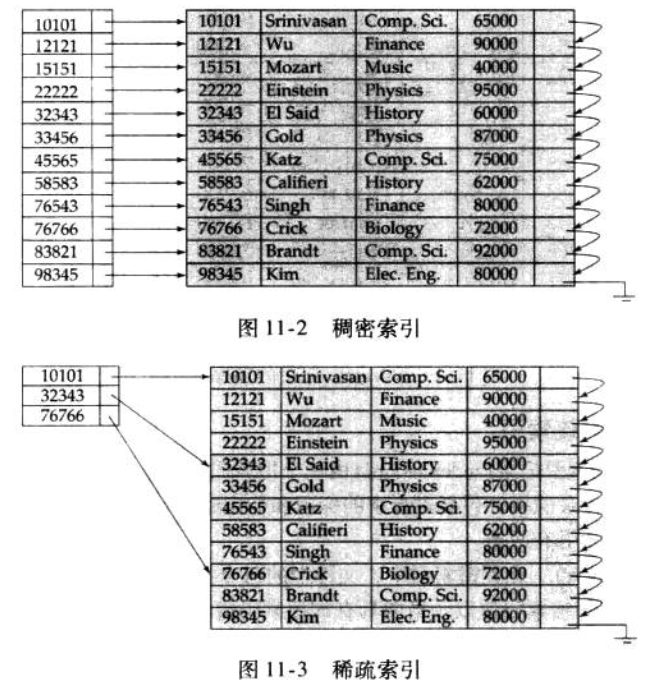
\includegraphics[width=0.6\linewidth]{fig/dense_sparse_indexing.png}
\end{figure}

通过建造多级稀疏索引,来减少访问时间。
\begin{figure}[H]
\centering
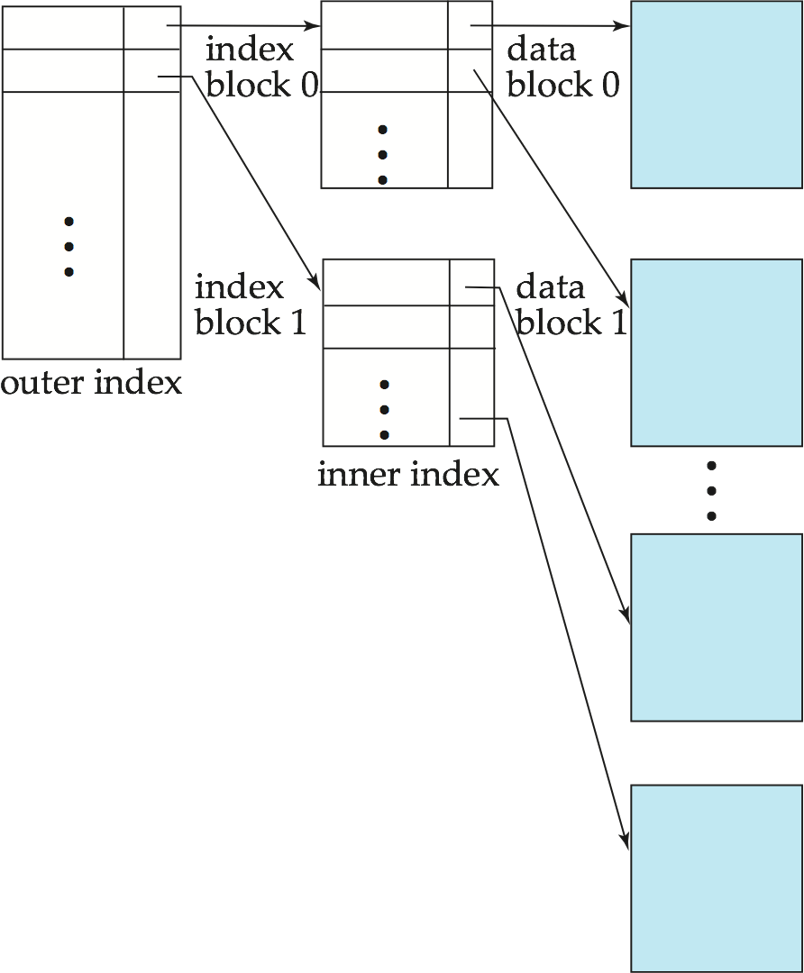
\includegraphics[width=0.4\linewidth]{fig/multilevel-index.png}
\end{figure}

索引更新操作:
\begin{itemize}
	\item 删除:稠密连同搜索码直接删,稀疏判大小
	\item 插入:同上直接插
\end{itemize}

\subsection{B+树索引}
当文件大起来时上述索引变得很慢,周期性更新整个文件非常麻烦,因此有B+树自动管理小的局部插入删除。

\subsubsection{基本性质}
B+树索引采用平衡树结构,树根到树叶的每条路径长度相同。
$n$-阶B树满足以下性质:
\begin{itemize}
	\item 所有叶子结点都必须在同一层
	\item 除了根结点外的\textbf{非叶子节点}都至少有$\lceil n/2\rceil$个孩子,至多$n$个孩子
	\item 叶子结点至少有\textcolor{red}{$\lceil (n-1)/2\rceil$}个关键字,最多$n-1$个关键字
	\item 特殊情况:
	\begin{itemize}
		\item 根节点不是叶子,则至少有$2$个孩子
		\item 根节点是叶子,则可以有$[0,n-1]$个值
	\end{itemize}
	\item 每个结点有$n$个指针,$n-1$个键值/搜索码\textbf{升序排序}(通常是严格不等式)
	\begin{center}
	\begin{tabular}{|c|c|c|c|c|c|c|}\hline
	$P_1$ & $K_1$ & $P_2$ & $\cdots$ & $P_{n-1}$ & $K_{n-1}$ & $P_n$\\\hline
	\end{tabular}
	\end{center}
	\item 左侧的叶子结点的搜索码值一定都小于\textbf{等于}右侧的叶子结点的搜索码值
	\item 指针与其\textbf{后面}的键值为一组,即$P_i$指向搜索码值为$K_i$的记录(叶子结点),或$P_i$指向$[K_{i-1},K_i)$(非叶子节点,注意右侧不包含);$P_n$指向下一个叶子节点
\end{itemize}

而B+树则是将所有关键字存储在叶子结点,其他结点作为索引,并且为每个叶子结点增加一个链指针。
\begin{figure}[H]
\centering
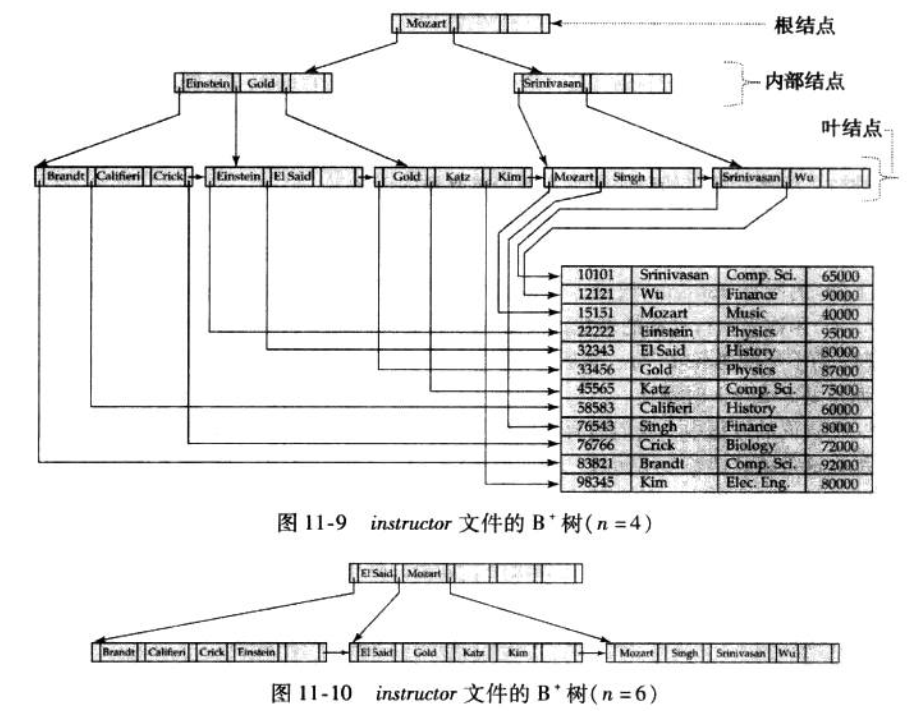
\includegraphics[width=0.6\linewidth]{fig/bp-tree.png}
\end{figure}

根节点下至少有$2\lceil n/2\rceil$个键值,下一层至少$2\lceil n/2\rceil^2$个,以此类推;
若记录中有$K$个搜索码值,则B+树树高不会高过$\lceil\log_{\lceil n/2\rceil}(K)\rceil$。

% 重复?

% https://blog.csdn.net/sunshine_lyn/article/details/82747596
\subsubsection{插入}
对于叶子节点的插入\footnote{B+树的动态演示可见\url{https://www.cs.usfca.edu/~galles/visualization/BPlusTree.html}}:
\begin{itemize}
	\item 搜索码值已经存在于叶子结点:直接加记录
	\item 搜索码值没有出现,添加记录到主文件,插入到叶子节点;如果没有位置,需要进行分裂
	\begin{itemize}
		\item 将这$n$个$(\text{搜索码值},\text{指针})$进行排序,取前$\lceil n/2\rceil$个在原来节点,其余在新节点
		\item 令新节点为$p$,$k$为$p$中的最小值,则插入\textemph{$(k,p)$}到父亲中,$p$为$k$的后续指针
		\item 若父亲满了,则继续分裂并传播
	\end{itemize}
\end{itemize}
\begin{figure}[H]
\centering
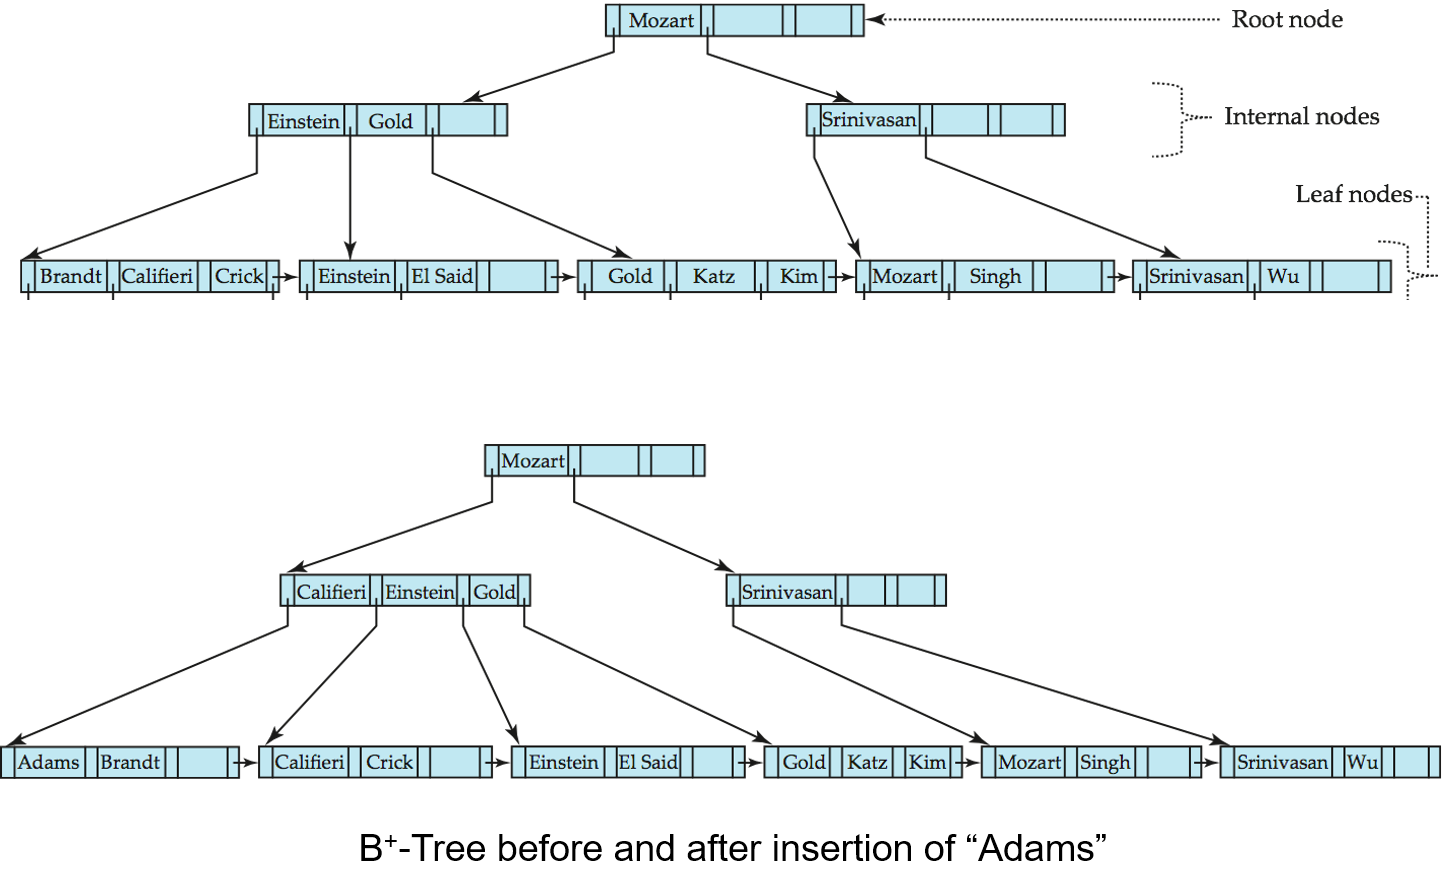
\includegraphics[width=0.8\linewidth]{fig/bp-tree_insertion.png}
\end{figure}

对于非叶子节点,当插入$(k,p)$到一个已经满的内部节点时:
\begin{itemize}
	\item 将$P_1,K_1,\ldots,K_{\lceil n/2\rceil-1},P_{\lceil n/2\rceil}$放到第一个节点
	\item 将$P_{\lceil n/2\rceil+1},K_{\lceil n/2\rceil+1},\ldots,K_n,P_{n+1}$放到第二个节点
	\item 将$(K_{\lceil n/2\rceil},N')$插入到父节点$N$
\end{itemize}
\begin{figure}[H]
\centering
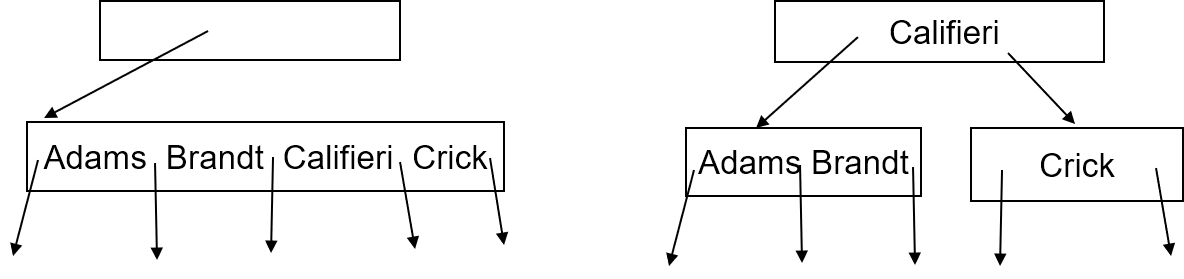
\includegraphics[width=0.6\linewidth]{fig/bp-tree_insertion3.png}
\end{figure}
\begin{figure}[H]
\centering
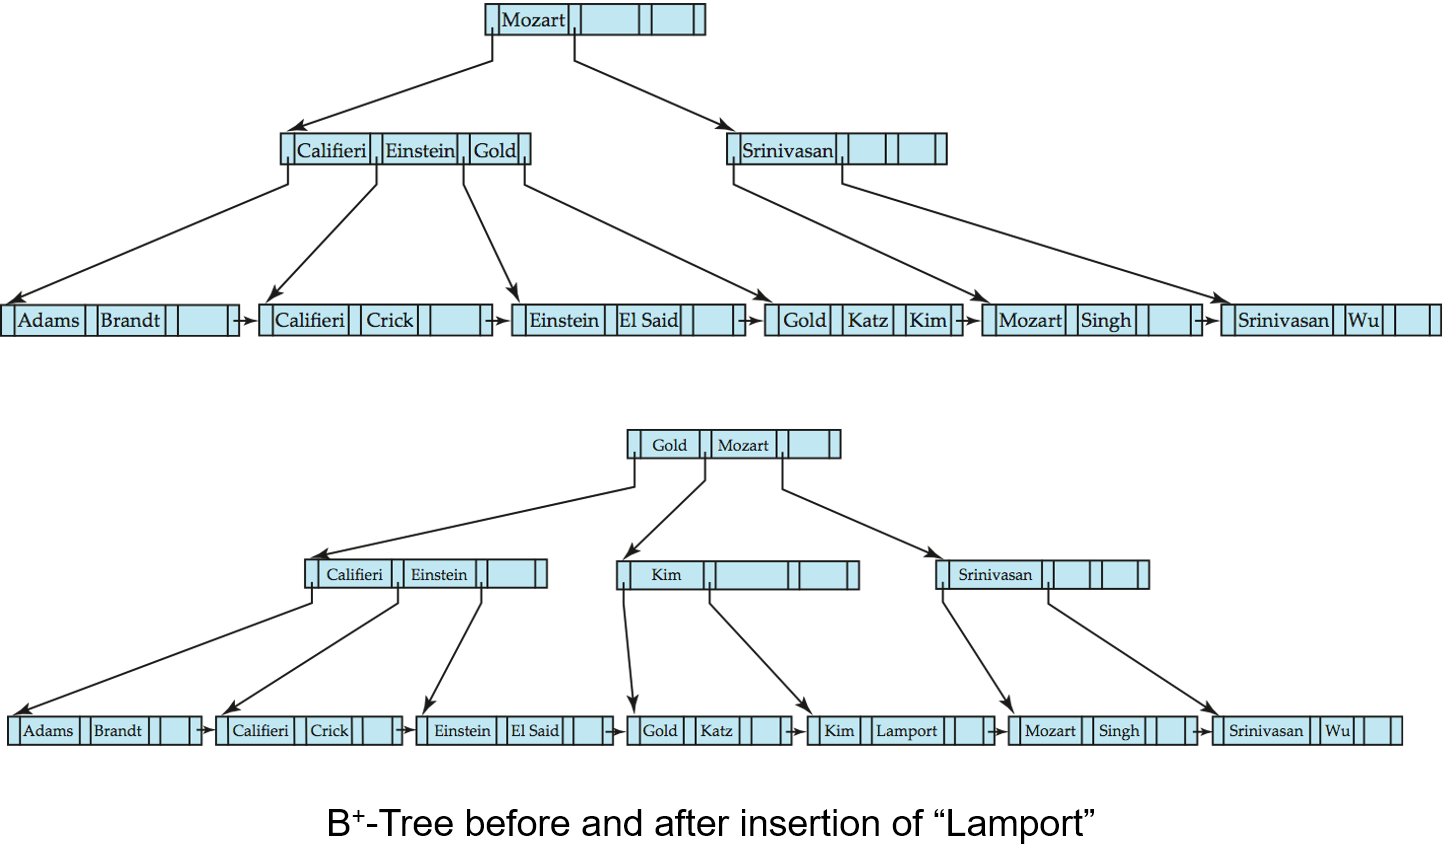
\includegraphics[width=0.8\linewidth]{fig/bp-tree_insertion2.png}
\end{figure}

\subsubsection{删除}
\begin{itemize}
	\item 直接移除
	\item 如果删除导致下溢(underfull)且可合并到一个结点,则合并兄弟
	\begin{itemize}
		\item 若\textemph{兄弟节点}未满,则与兄弟节点合并(注意不是同层都是兄弟)
		\item 删除$(K_{i-1},P_i)$,其中$P_i$是指向删除结点的指针,更新索引值,递归这个过程
	\end{itemize}
	\item 如果合并没法合到一个节点,则需要\textbf{重分配}(redistribute)指针使得两个兄弟节点都含有多于最小键值数目的项,同时更新父亲节点的搜索码
\end{itemize}
\begin{figure}[H]
\centering
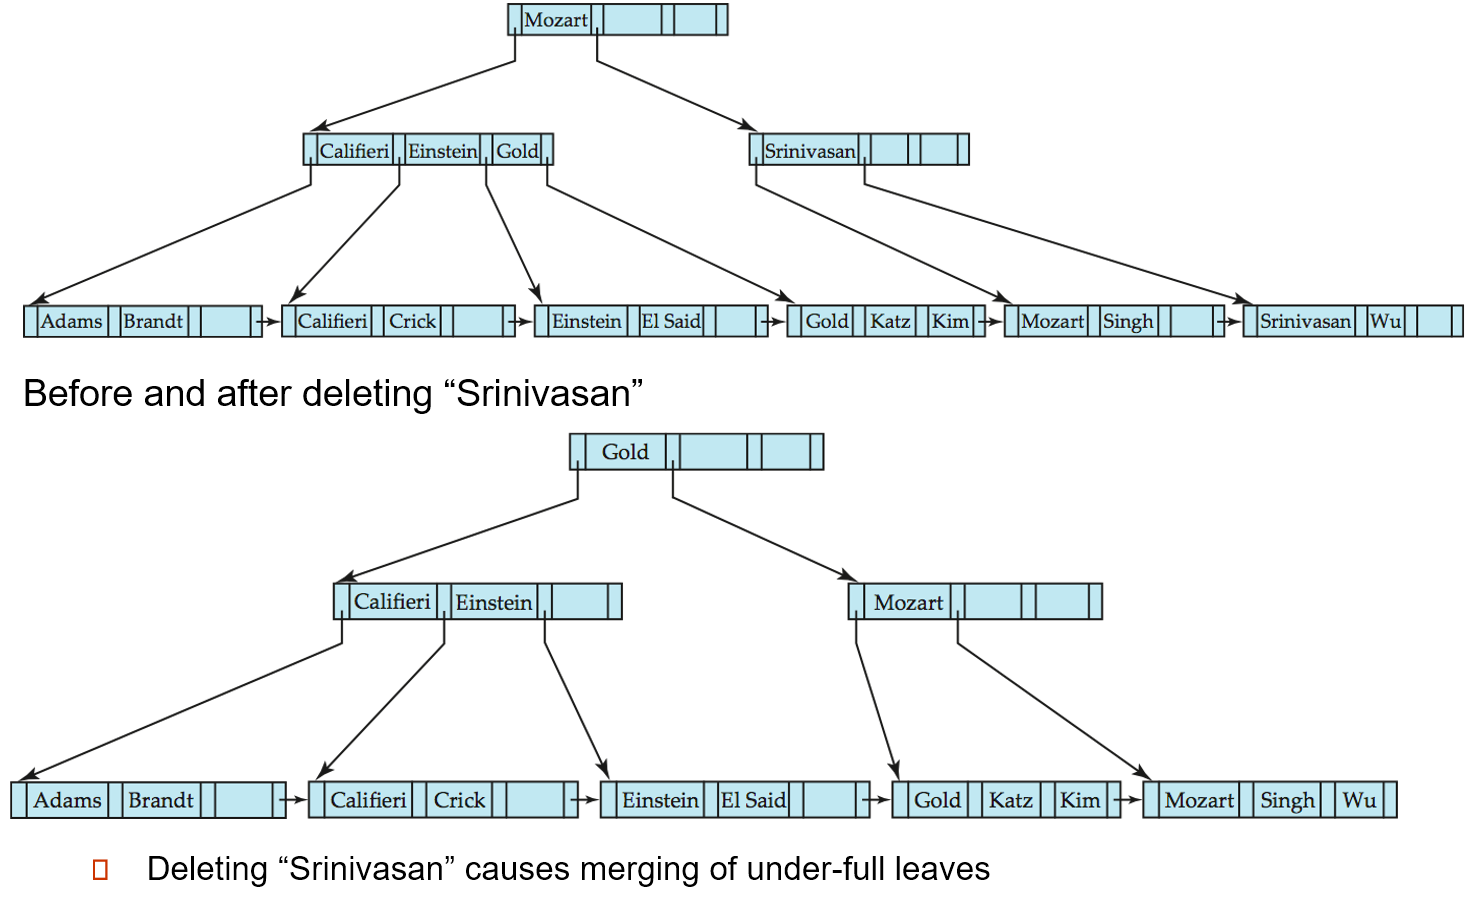
\includegraphics[width=0.8\linewidth]{fig/bp-tree_deletion.png}
\end{figure}
\begin{figure}[H]
\centering
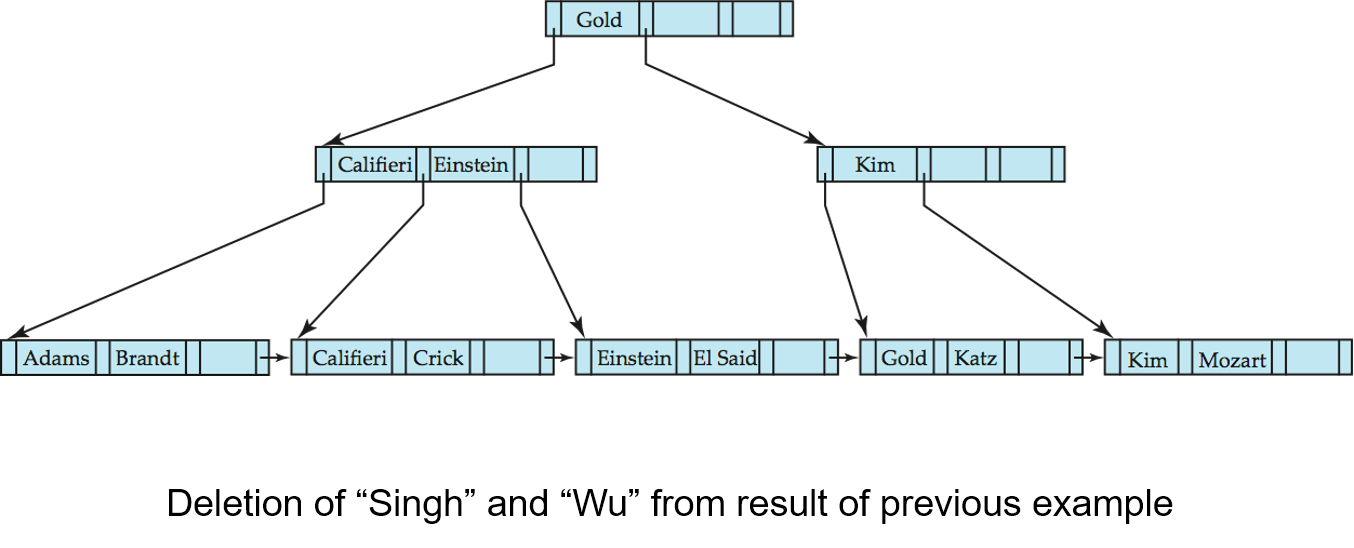
\includegraphics[width=0.8\linewidth]{fig/bp-tree_deletion2.png}
\end{figure}
\begin{figure}[H]
\centering
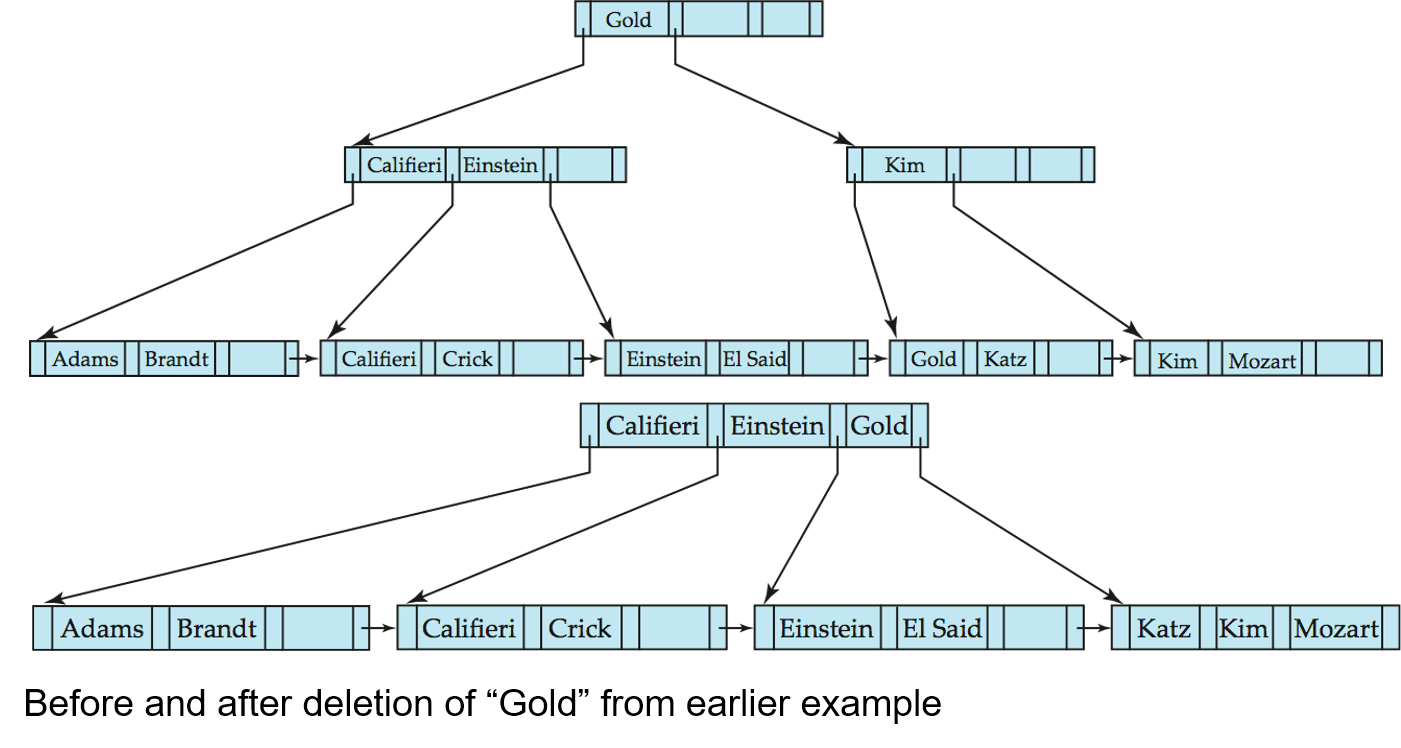
\includegraphics[width=0.8\linewidth]{fig/bp-tree_deletion3.png}
\end{figure}
\begin{figure}[H]
\centering
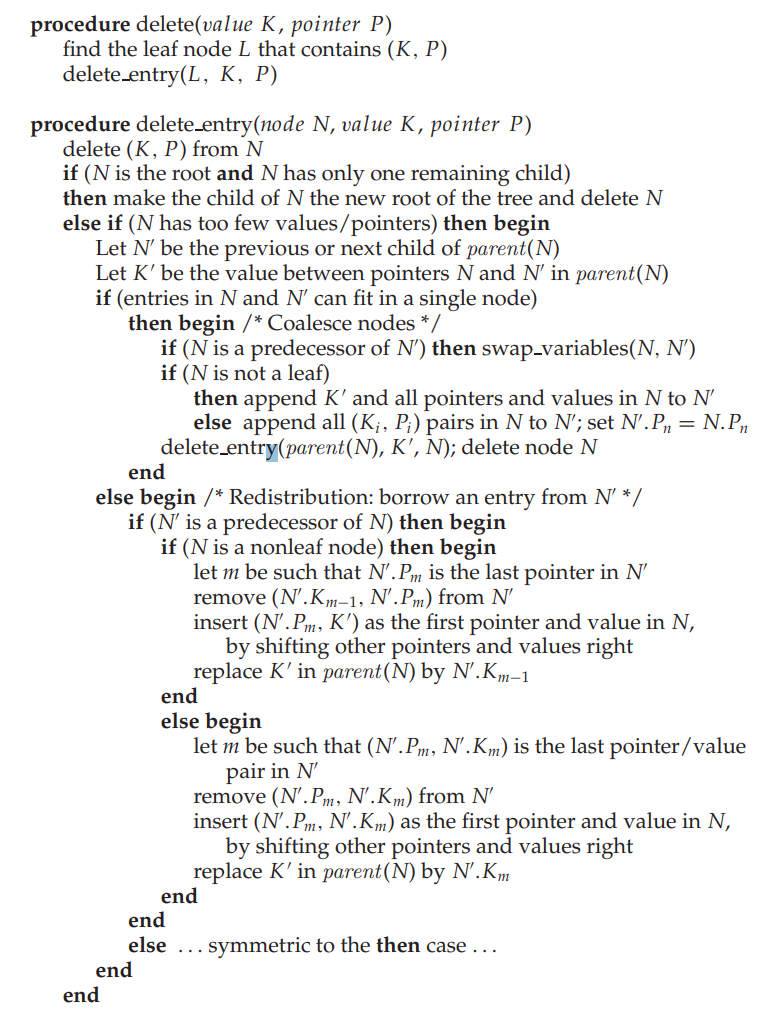
\includegraphics[width=0.7\linewidth]{fig/bp-tree_deletion_alg.png}
\end{figure}

\subsubsection{其他事项}
\begin{itemize}
	\item 前缀压缩:比如``abcde''和``abds''可以通过``ab''进行区分
	\item 多码索引:构成元组进行索引
\end{itemize}

\subsubsection{B+树文件组织}
\begin{figure}[H]
\centering
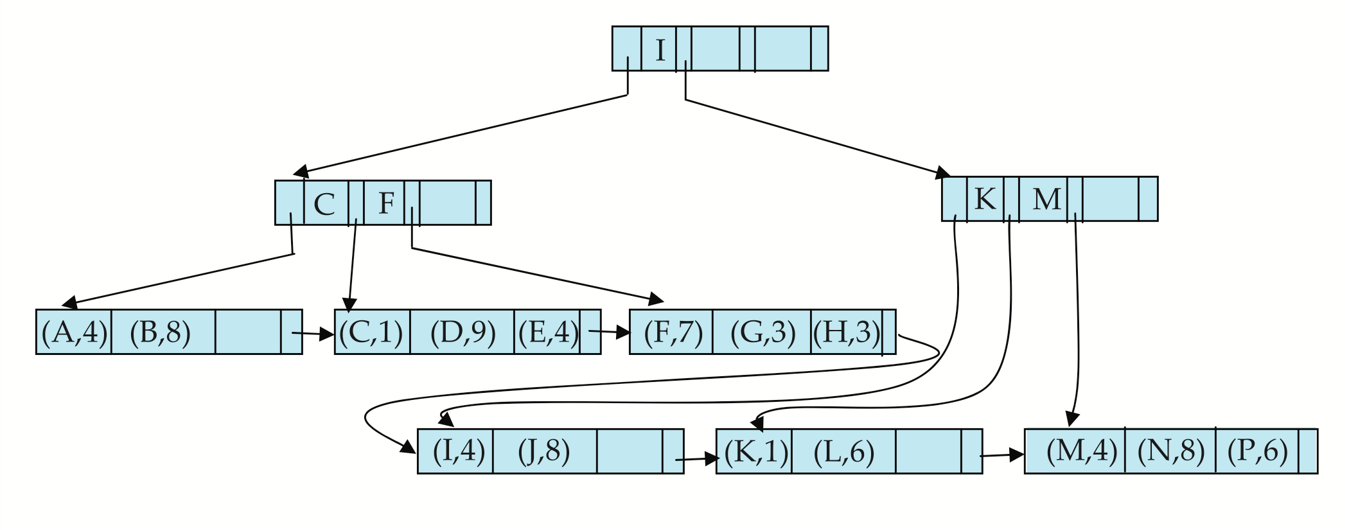
\includegraphics[width=0.8\linewidth]{fig/bp-tree_file_organization.png}
\end{figure}

\subsubsection{B树}
\begin{figure}[H]
\centering
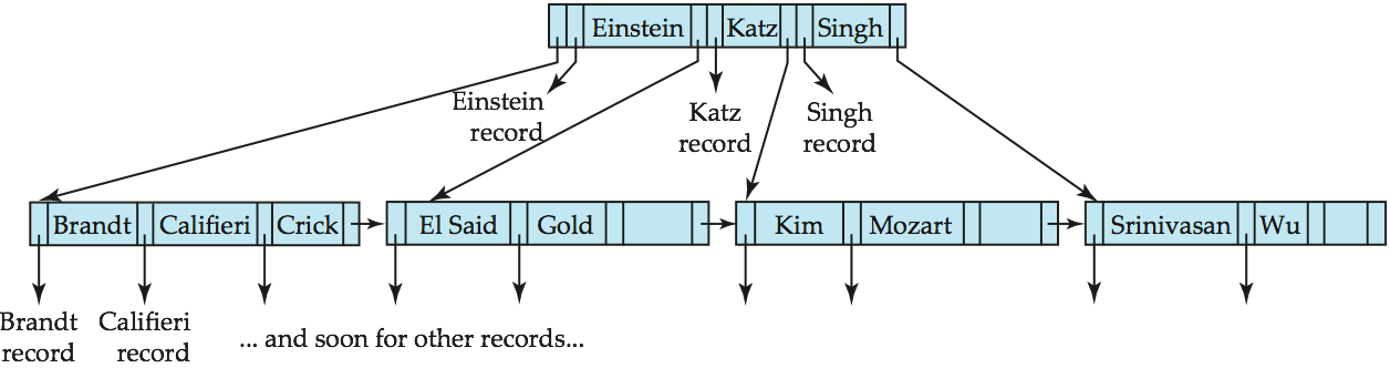
\includegraphics[width=0.8\linewidth]{fig/b-tree.png}
\end{figure}

\subsection{静态散列}
散列(hash)函数应该满足:
\begin{itemize}
	\item 分布均匀:为每个桶分配同样数量的搜索码值
	\item 分布随机:不应与搜索码的任何外部可见排序相关
\end{itemize}

两种散列结构:
\begin{itemize}
	\item 闭散列:一个桶的溢出桶都用链表链接在该桶后面形成溢出链(overflow chaining)
	\item 开散列:线性探查法(probing)插入到下一个有空间的桶
\end{itemize}

下例的散列函数为ID各位数字之和对8取模
\begin{figure}[H]
\centering
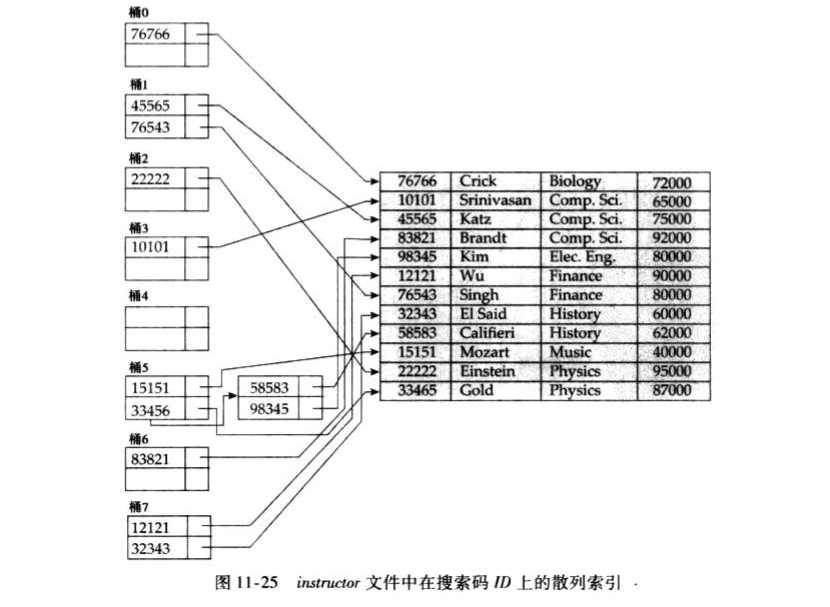
\includegraphics[width=0.8\linewidth]{fig/hash_index.png}
\end{figure}

静态散列问题:
\begin{itemize}
	\item 太小导致后期冲突多性能下降
	\item 太大则大量空间被浪费
\end{itemize}

\subsection{动态散列}
当数据库增大或缩小时,可扩充散列(extendable hashing)可通过桶的分裂或合并来适应数据库大小变化。

通常选择一个具有均匀性和随机性特性的散列函数$h$,且产生范围较大,是$b$位二进制整数,通常$b=32$。
通过哈希函数的前$i$位确定索引,每次桶满了才考虑新增一位,且不到万不得已不分裂(原来前缀相同的全指向同一个桶)。
但如果散列值相同,则只能采用溢出桶的方法。
\begin{figure}[H]
\centering
\begin{tabular}{cc}
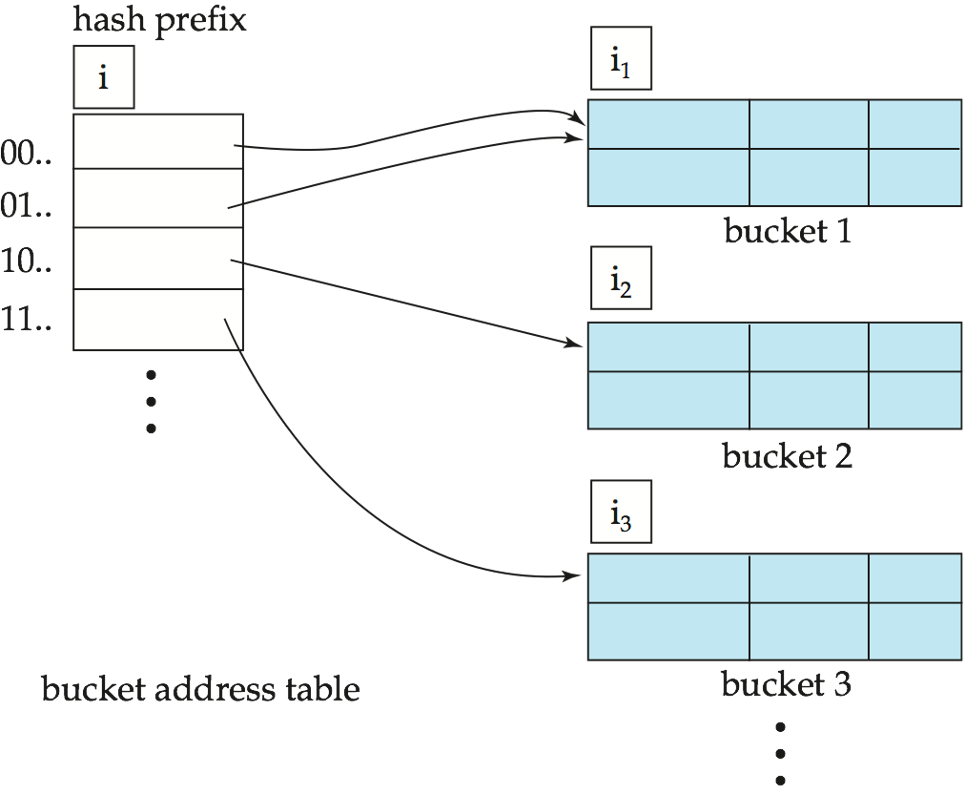
\includegraphics[width=0.5\linewidth]{fig/extendable_hash.png}&
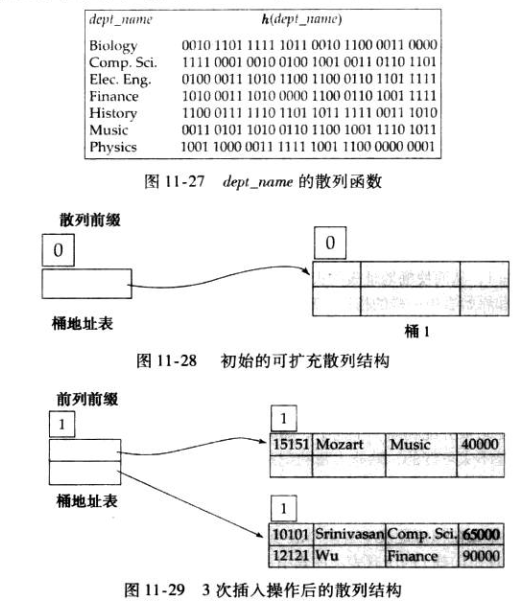
\includegraphics[width=0.5\linewidth]{fig/extendable_hash_eg.png}
\end{tabular}
\end{figure}
但缺点在于查找涉及一个附加的间接层,系统在访问桶本身之前必须先访问桶地址表。

\subsection{位图索引}
一共是元组个数$n$位,若第$i$个元组的该属性为某特定值,则设为1,否则置0。
\begin{figure}[H]
\centering
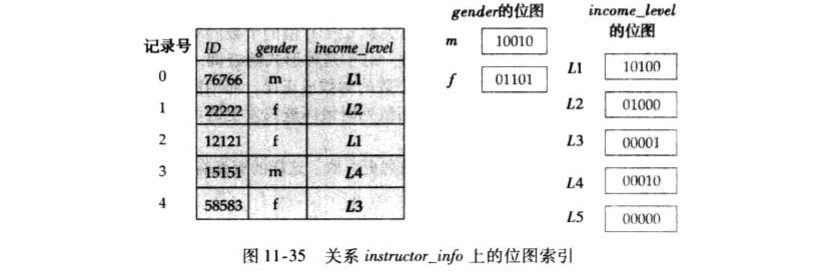
\includegraphics[width=0.9\linewidth]{fig/bitmap.png}
\end{figure}